\def\cvprPaperID{9284}
\def\confName{ICCV}
\def\confYear{2023}

\def\paperTitle{Deformable Neural Radiance Fields using RGB and Event Cameras}

\def\authorBlock{
    Author 1\thanks{Equal contribution} \qquad
    Author 2\footnotemark[1] \qquad
    Author 3 \\
    Institute \\
    {\tt\small \{email, addresses\}@inst.edu}
}

% Compilation vars
\newif\ifreview \newcommand{\review}{\reviewtrue}
\newif\ifarxiv \newcommand{\arxiv}{\arxivtrue}
\newif\ifcamera \newcommand{\cameraready}{\cameratrue}
\newif\ifrebuttal \newcommand{\rebuttal}{\rebuttaltrue}

\review % \review OR \cameraready

\documentclass[10pt,twocolumn,letterpaper]{article}
\input{cvpr_header}

\myexternaldocument{_main}
\begin{document}

%% TITLE
\title{\paperTitle \\ Supplemental Material}
\author{\authorBlock}
\maketitle
%%
\renewcommand\thesection{\Alph{section}}
%\section{Structure of this document}
In this document, we provide additional details of our method and implementations. We further provide more qualitative and some quantitative results. Please also refer to the supplementary video for additional qualitative visualizations. 


\section{Video Interpolation using Events for NeRF}
The usage of event cameras in computer vision has been motivated by their unique advantages, namely, high dynamic range, low latency, ultra-low power consumption, and the absence of motion blur. \cite{tulyakov2021time} take advantage of synthesis-based and flow-based approaches which are robust to motion blur. \cite{lin2020learning} propose using the dynamic filtering layer to address the spatially variant threshold and represent the residuals between a blurry image and sharp frames as integrals of events \cite{pan2019bringing}. \cite{zhang2022unifying} introduces a unified framework for event-based video deblurring and interpolation using a double integral (LDI) network and a fusion network. \cite{paikin2021efi} propose a novel three-phase CNN architecture that fuses intensity images and event stream first at event camera resolution and then scales up to RGB resolution, followed by colorization. \cite{wang2020eventsr} deploys adversarial learning to reconstruct HR intensity images from LR event streams. Unlike the mentioned works,  we do not interpolate the video frames and then train the deformation neural radiance Field upon them. Instead, we process the asynchronous events in their raw form which brings us computational efficiency while exploiting the temporal precision of events.



%Our method uses asynchronous event information instead of synchronized interpolated frames, while the aforementioned methods require the specification of upsampled frame timestamps. We focus on deformation-induced events rather than all frame spatial information, reconstructing the whole image is redundant. 

\section{Details of Synthetic Data}
In this section, we provide additional details of the campfire and fluids dataset, created by us. The campfire and fluids datasets are made from Blender models. To simulate realistic fire and fluid in high framerate we set 960fps in Blender. The resolution of fire is $128^3$ while for fluids is $320^3$. We decrease the reaction speed for the campfire to 0.8 and increase the maximum temperature to 3.1 to control the flames rising speed. Turbulence is also introduced to bring uncertainty to the flaming process. For fluids, we increase the particle sampling per cell to better simulate the motion of water. More details such as customized shading can be found in the Blender file of our dataset, which we will make available.

\section{Details of PoseNet}
Recall that in Section 3, we encode the pose residual term through screw axis representation:  $\mathsf{S}=(r(t);v(t)) \in \mathbb{R}^{6} $. We train 2 MLPs which output $r(t) \in \mathbb{R}^{3}, v(t) \in \mathbb{R}^{3} $ after encoding time using sinusoidal positional encoding similar to the input coordinate $ \gamma(t): \mathbb{R}^{1} \rightarrow \mathbb{R}^{1+\theta m} $. This allows the network to learn high-frequency representation from time input. We choose $m = 1$ for PoseNet and also for encoding time in the deformation network. Next, we calculate the translation and rotation using Rodrigues' rotation formula
$\mathsf{R} = \mathsf{I} + \sin\theta\mathsf{K} + (1-\cos\theta)\mathsf{K}^2$
where $\mathsf{R}$ is the rotation matrix, $\theta$ is the rotation angle which can be calculated by $\theta = \lVert r(t)  \rVert$, and $\mathsf{K}$ is a skew-symmetric matrix also known as the cross product matrix of the unit vector $ \hat{r}(t)  = \frac{r(t)}{\lVert r(t)  \rVert}$. We can also compute the translation vector as: 
$$\mathbf{v} = \frac{(1-\cos(\theta))(\mathbf{\hat{r}}\times\mathbf{v}) + \sin(\theta)\mathbf{\hat{r}}\times(\mathbf{\hat{r}}\times\mathbf{v}) + \cos(\theta)\mathbf{v}}{\theta^2},$$

As mentioned in Section 3.1,  the PoseNet learns the pose residuals. Here, we compare the results for learning to pose residual and absolute pose, which are presented in Table \ref{tab:different_pose}. It is expected that learning residual yields better results as the initialized pose will be closer to the ground truth pose.

\begin{table}[!htbp]
\begin{center}
\resizebox{0.8\linewidth}{!}{
\begin{tabular}{lcccc}
\toprule
Lego & MSE & PSNR & SSIM & LPIPS \\
\midrule
Pose residual & 0.32 & 35.04 &0.99 & 0.03\\
Pose absolute & 2.18 & 26.09 & 0.96  & 0.151  \\
\bottomrule
\end{tabular}}
\vspace{1mm}
\caption{\textbf{Absolute pose vs. residual pose.} In the upper row the PoseNet is trained to learn the residual from the interpolated poses using RGB frame poses, while the bottom row is trained to learn the pose directly. 
}
\label{tab:different_pose}
\end{center}
\end{table}

Recall that in Figure 5 of the main paper we provide the position error obtained by initial pose interpolation. Here in Figure~\ref{fig:roation_error} we report the rotation error of our method after injecting different magnitudes of rotation noise. We found that our method is robust to small rotation noise and can effectively reduce large rotation noise.



\begin{figure}
    \centering
    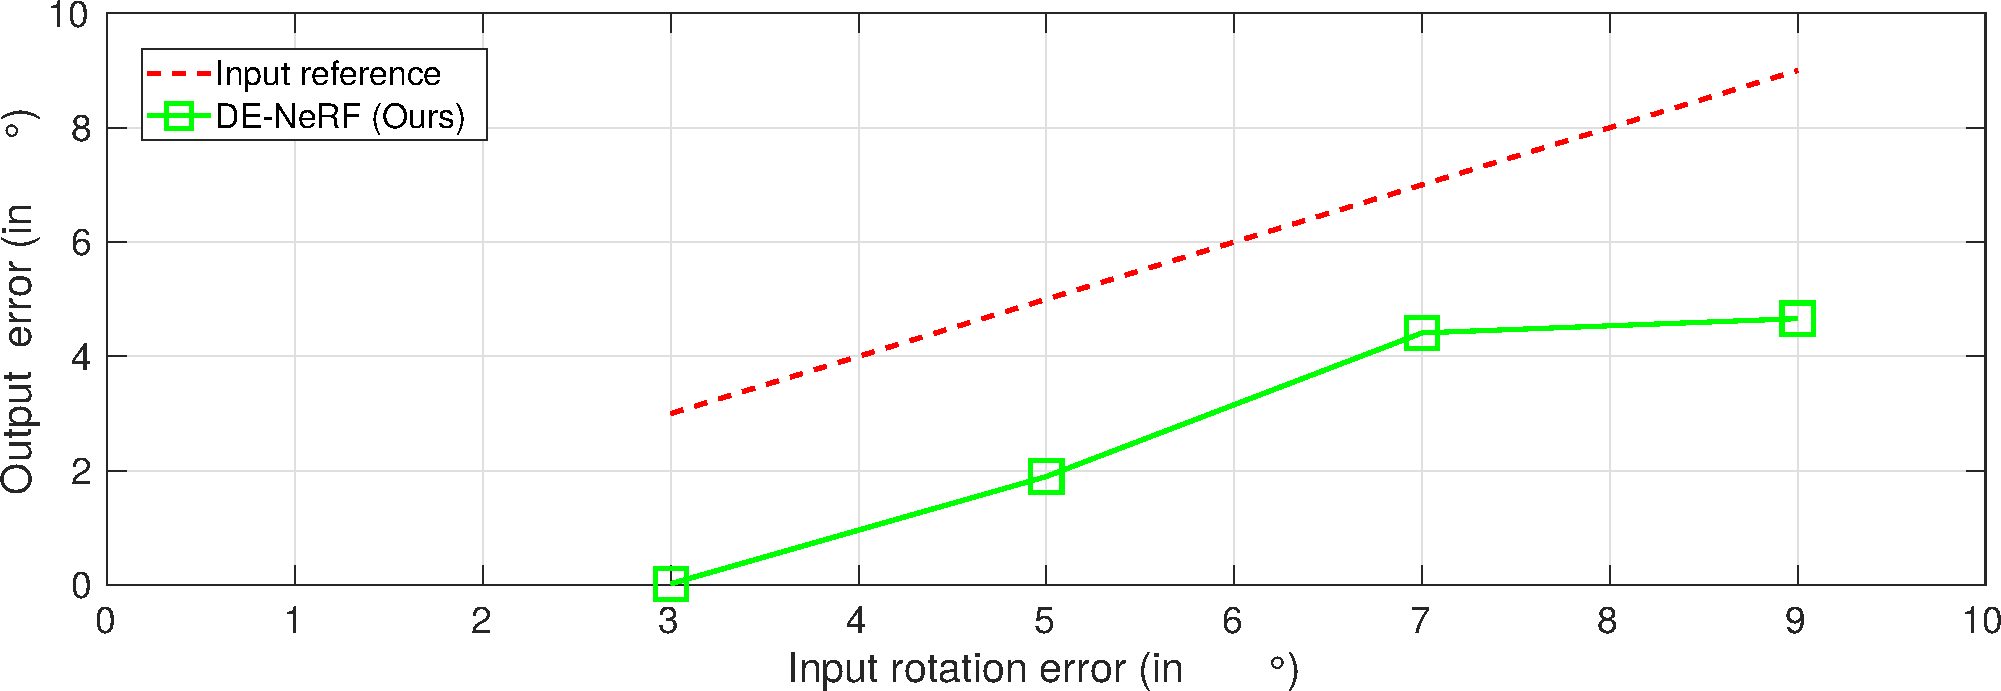
\includegraphics[width=0.960\linewidth]{rotation_error.pdf}    
    \caption{{PoseNet robustness against injected rotation noise.} }
    \label{fig:roation_error}
\end{figure}

%\begin{table}[!htbp]
%\begin{center}
%\resizebox{0.6\linewidth}{!}{
%\begin{tabular}{lcccc}
%\toprule
%Lego &  &  &  &  \\
%\midrule
%Rotation Error inject & 3 & 5 & 7 & 10 \\
%Pose Error & - & - & -  & -  \\
%\bottomrule
%\end{tabular}}
%\vspace{1mm}
%\caption{\textbf{PoseNet against rotation error injection.}
%}
%\label{tab:Rotation error}
%\end{center}
%\end{table}

% \todo[inline]{change this to plots}
% \todo[inline]{The events used should expressed in 10^6}


\begin{table}[h]
\resizebox{\linewidth}{!}{
\begin{tabular}{lcccccc}
\toprule
 Number of Views & \multicolumn{2}{c}{10} & \multicolumn{2}{c}{25} & \multicolumn{2}{c}{50}  \\
\cmidrule(r){2-3} \cmidrule(r){4-5} \cmidrule(r){6-7}
Metinaccurately & LPIPS & PSNR & LPIPS & PSNR & LPIPS \\
\midrule

Train from scratch & 30.06  & 0.0623  & 33.95 & 0.045 & 35.45 & 0.036 \\
Finetune & 32.13 & 0.046  & 32.55  & 0.037 & 35.04 & 0.034 \\
% Finetune on RGB+Events & - & - & - & - & -  & - \\

\bottomrule
\end{tabular}}
\vspace{1mm}
\caption{\textbf{Training Protocol.} Training from scratch provide better results with more accurate pose initialization but for inaccurate pose initialization training PoseNet as finetuning after a first round of training performs better.
}
\label{tab:training_protocal}
\end{table}

\section{More Details on Implementation \& Training}

We first dive into more details about the implementation of our DE-NeRF and then provide the training protocols and hyperparameters.% and then we will discuss the training protocol and hyperparameters.
We initialize the radiance field MLP with Xavier-initialization and similar to \cite{park2021nerfies} for both deformation and PoseNet we initialize the output layer with uniform distribution from $ \mathcal{U}( -10^{-4},10^{-4} )$ so that the transformation will initially remain close to identity.
The optimizer for training both the deformation radiance Field and the PoseNet are Adam \cite{kingma2014adam}: $\beta_1 = 0.9$ and $\beta_2 = 0.999$. The learning rate 
follows an exponentially decayed schedule from 2e-3 to 1e-4. For PoseNet the learning rate decayed from 1e-3 to 5e-5 for stable training.
% $2^{-3}$

Here we compare two different training protocols in \textbf{Non-rigid Lego} with a different number of frames used as shown in Table \ref{tab:training_protocal}. Train from scratch implies that DE-NeRF learns the radiance field as well as the trajectory residual at the same time from the beginning. In contrast, the Finetune approach learns the deformation radiance field only based on the interpolated trajectory and then enables the PoseNet later for joint training. We found that when the pose is well-initialized, using 25 and 50 frames, better results are obtained when enabling PoseNet in the beginning. Conversely, when the initialized pose inaccurately for 10 frames cases, we found enabling the PoseNet after a pre-training improves the results. It can be attributed to the benefits of solving tasks one by one and the learned radiance field provides additional constraints for PoseNet training.

\begin{table}[h]
\begin{center}
\resizebox{0.7\linewidth}{!}{
\begin{tabular}{lcccc}
\toprule
$\lambda$ & MSE & PSNR & SSIM & LPIPS \\
\midrule
100 & 0.54 & 33.59 & 0.993 & 0.0429 \\
10 & 0.30 & 35.44 & 0.997 & 0.0363\\
1 & 0.32  & 35.02 & 0.995 & 0.0533  \\
0.1 & 1.02 & 30.24  & 0.981  & 0.0929  \\
0.01 & 6.13 & 22.20  & 0.873  &  0.3124 \\
\bottomrule
\end{tabular}}
\vspace{1mm}
\caption{\textbf{Influence of $\lambda$.} PSNR values for different hyperparameter $\lambda$ of the RGB photometric loss on Lego dataset.
}
\label{tab:lambda_compare}
\end{center}
\end{table}

\begin{table}[!htbp]
\begin{center}
\resizebox{0.8\linewidth}{!}{
\begin{tabular}{lcccc}
\toprule
Lego & MSE & PSNR & SSIM & LPIPS \\
\midrule
Translation & 0.32 & 35.04 &0.99 & 0.03\\
SE(3) & 0.33 & 34.57 & 0.99  & 0.052  \\
\midrule
Umbrella & MSE & PSNR & SSIM & LPIPS \\
\midrule
Translation & 0.45  & 33.44 & 0.95 & 0.341  \\
SE(3) & 0.37 & 33.99  & 0.95  & 0.342  \\
\bottomrule
\end{tabular}}
\vspace{1mm}
\caption{\textbf{Different warps.} Two cases highlighting the pros and cons of SE(3) deformation field compared to translation only.
}
\label{tab:rotation_compare}
\end{center}
\end{table}



\newcolumntype{C}{ >{\centering\arraybackslash} p{0.16\linewidth} }

\begin{table*}
\begin{center}
\begin{tabular}{ @{}rC@{\hskip 3pt}C@{\hskip 3pt}C@{\hskip 3pt}C@{\hskip 3pt}C@{} }
%{ccccccc}
\vspace{-0.5cm}
\rotatebox{90}{Lego} &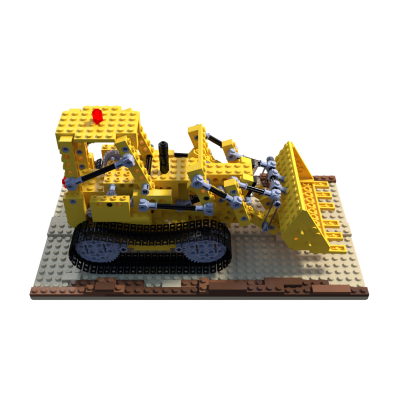
\includegraphics[width=\linewidth,valign=m]{figs/depth_compare_big/lego/lego000500_gt.png} & 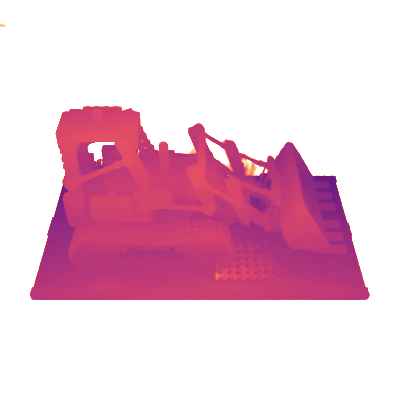
\includegraphics[width=\linewidth,valign=m]{figs/depth_compare_big/lego/lego_depth_ours.png}  & 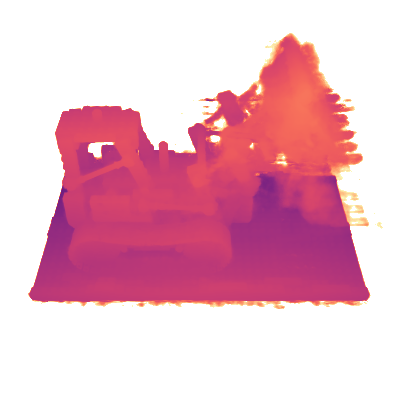
\includegraphics[width=\linewidth,valign=m]{figs/depth_compare_big/lego/lego_depth_enerfie.png} & 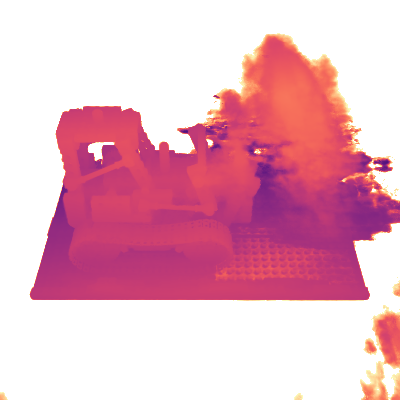
\includegraphics[width=\linewidth,valign=m]{figs/depth_compare_big/lego/lego_depth_nerfie.png} & 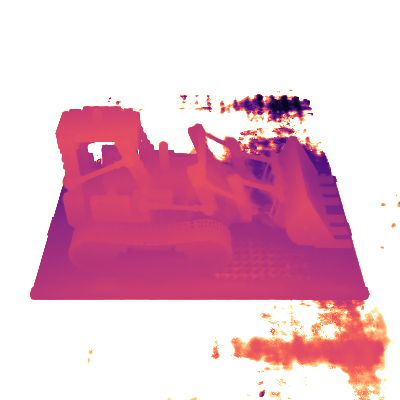
\includegraphics[width=\linewidth,valign=m]{figs/depth_compare_big/lego/lego_depth_hypernerf.png} \\

\vspace{-0.2cm}
\rotatebox{90}{Campfire} & 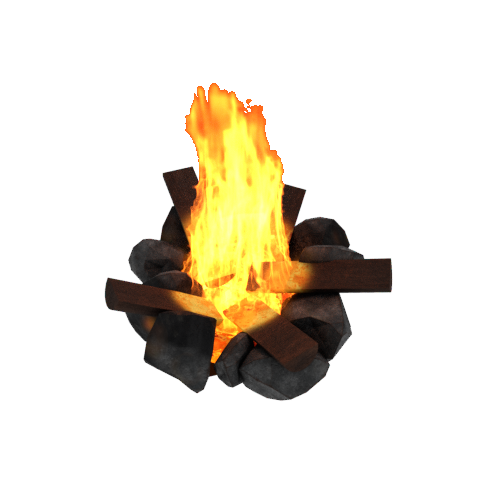
\includegraphics[width=\linewidth,valign=m]{figs/depth_compare_big/campfire/000007.png} & 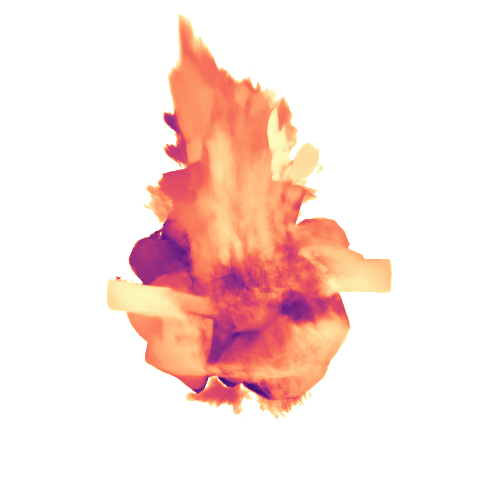
\includegraphics[width=\linewidth,valign=m]{figs/depth_compare_big/campfire/fire_depth_ours.png} & 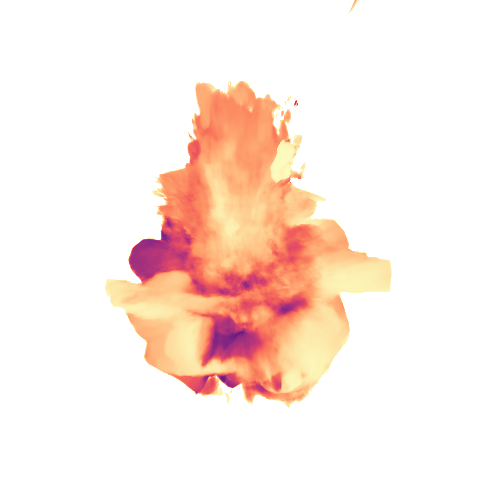
\includegraphics[width=\linewidth,valign=m]{figs/depth_compare_big/campfire/fire_depth_enerfie.png} & 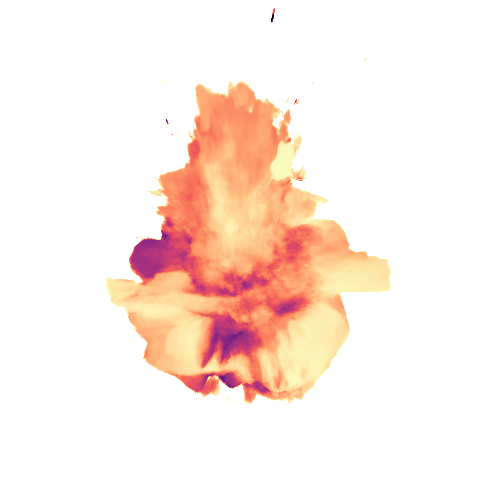
\includegraphics[width=\linewidth,valign=m]{figs/depth_compare_big/campfire/fire_depth_nerfies.png} & 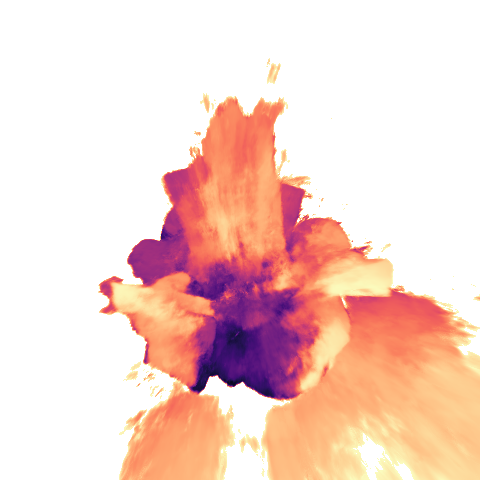
\includegraphics[width=\linewidth,valign=m]{figs/depth_compare_big/campfire/fire_depth_hypernerf.png}  \\

\vspace{0.1cm}

\rotatebox{90}{Fluid} &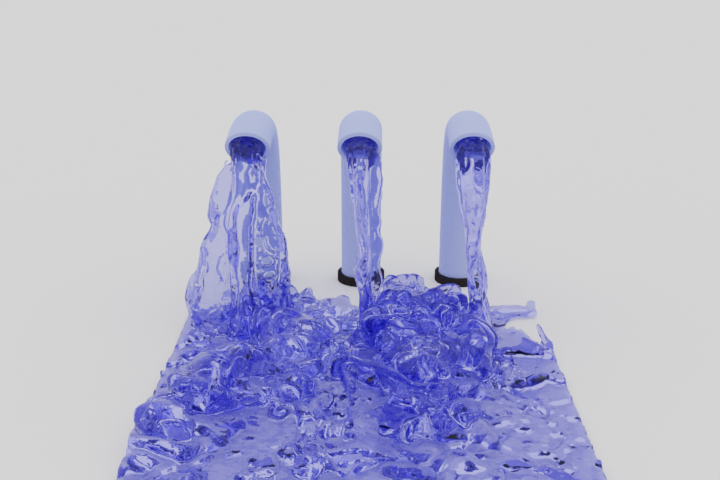
\includegraphics[width=\linewidth,valign=m]{figs/depth_compare_big/fluid/000706.png} & 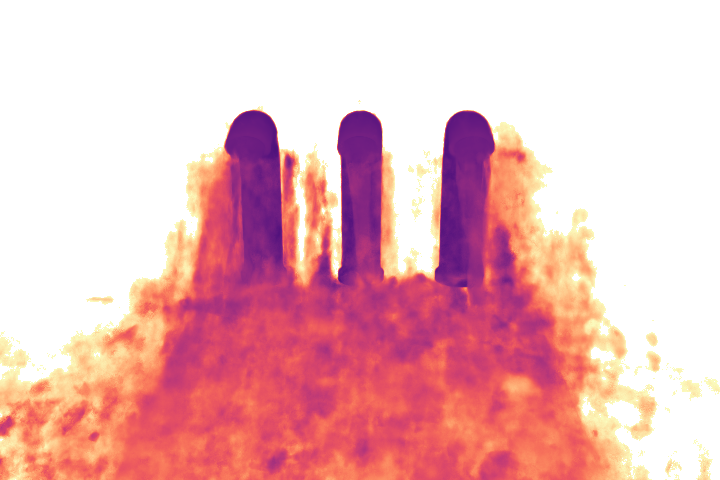
\includegraphics[width=\linewidth,valign=m]{figs/depth_compare_big/fluid/fluid_depth_denerf.png} & 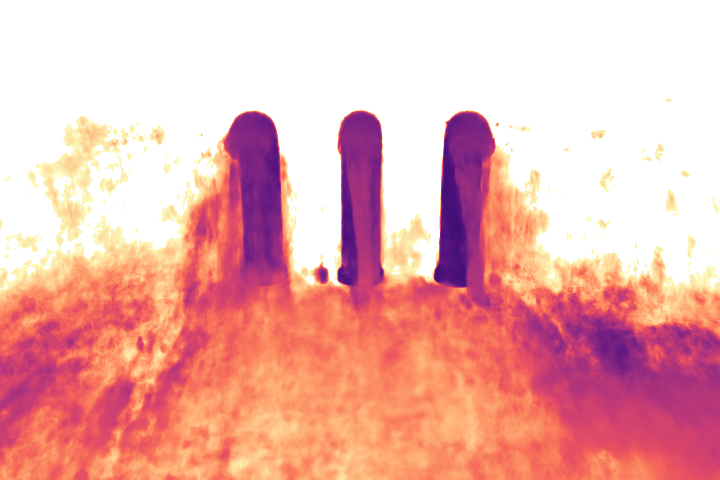
\includegraphics[width=\linewidth,valign=m]{figs/depth_compare_big/fluid/fluid_depth_enerfie.png} & 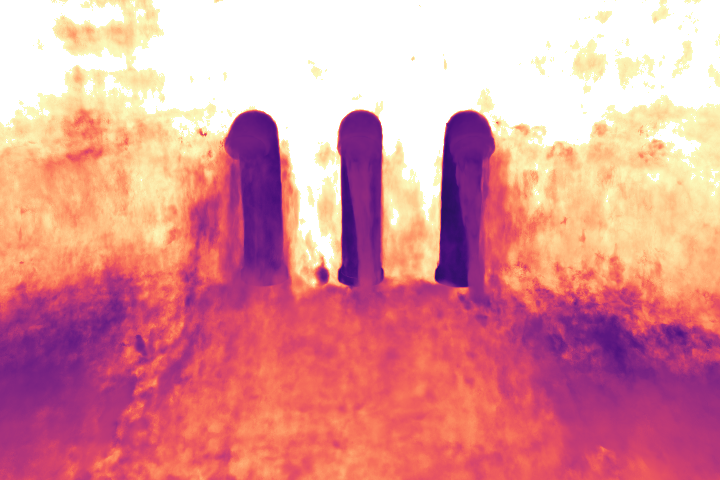
\includegraphics[width=\linewidth,valign=m]{figs/depth_compare_big/fluid/fluid_depth_nerfies.png} & 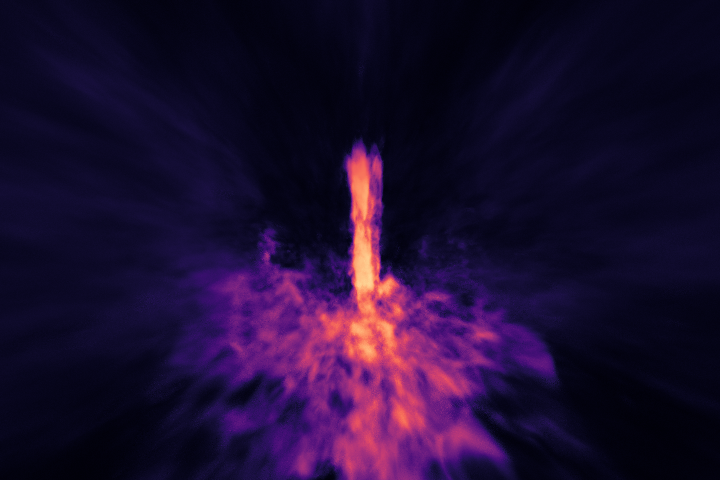
\includegraphics[width=\linewidth,valign=m]{figs/depth_compare_big/fluid/fluid_depth_hypernerf.png}  \\

\vspace{0.1cm}
\rotatebox{90}{Umbrella} & 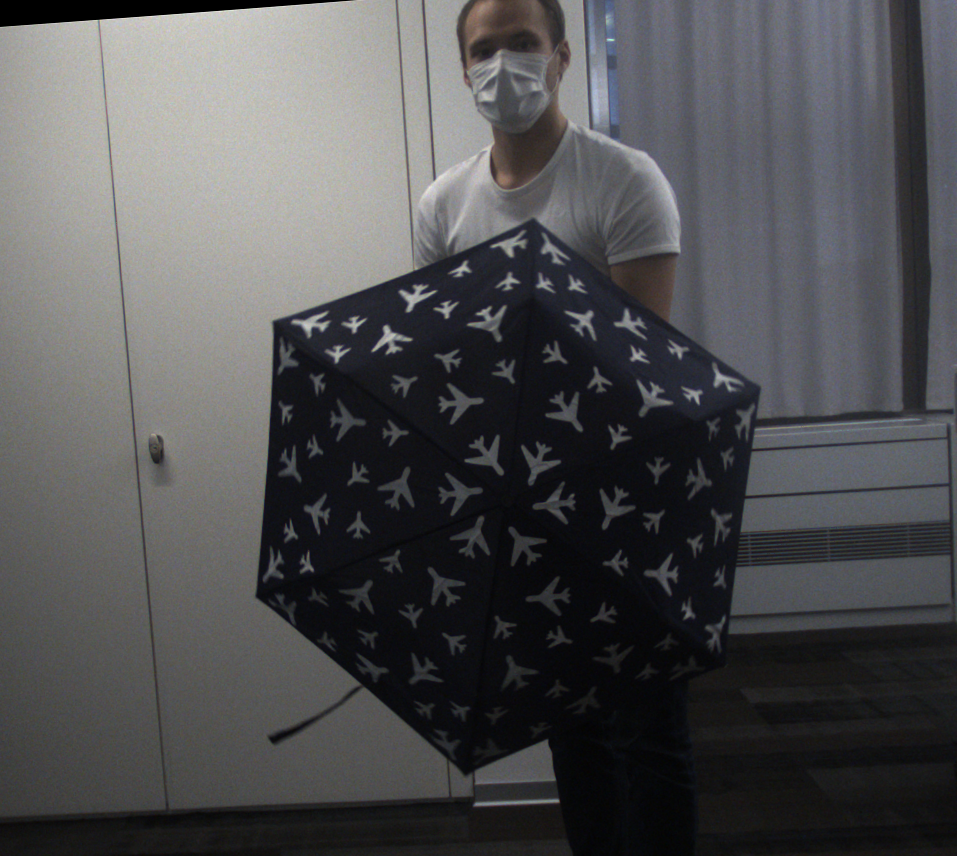
\includegraphics[width=\linewidth,valign=m]{figs/depth_compare_big/umbrella/000150.png} & 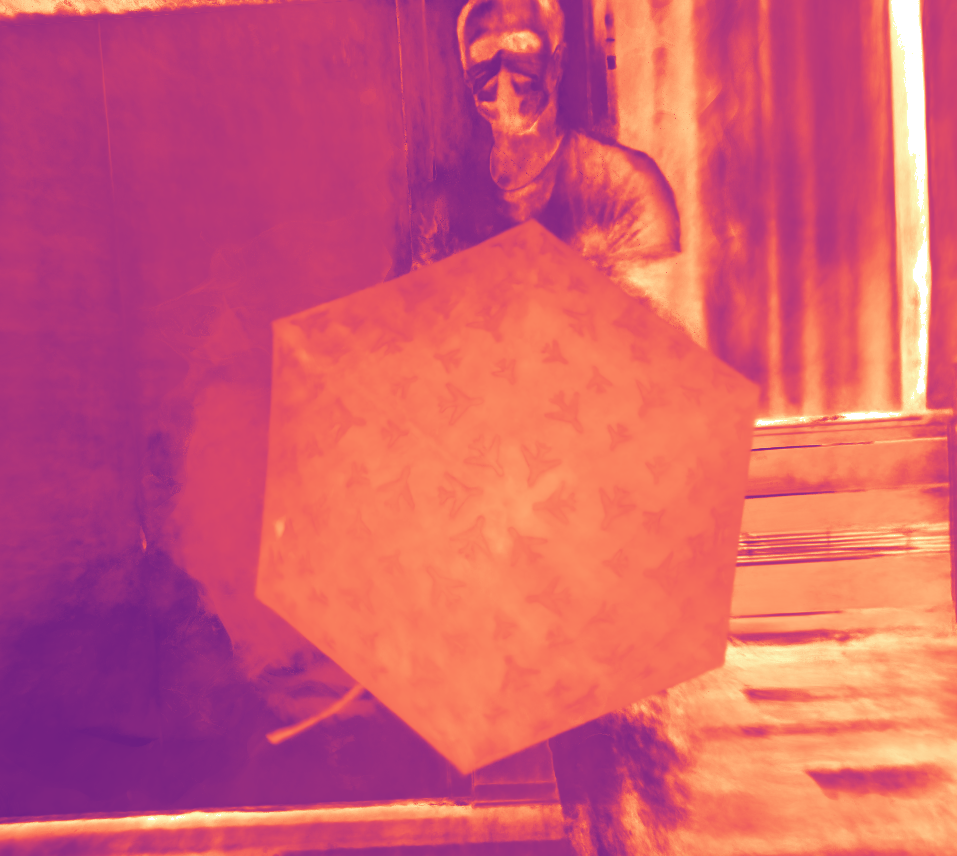
\includegraphics[width=\linewidth,valign=m]{figs/depth_compare_big/umbrella/umbrella_denerf_depth.png} & 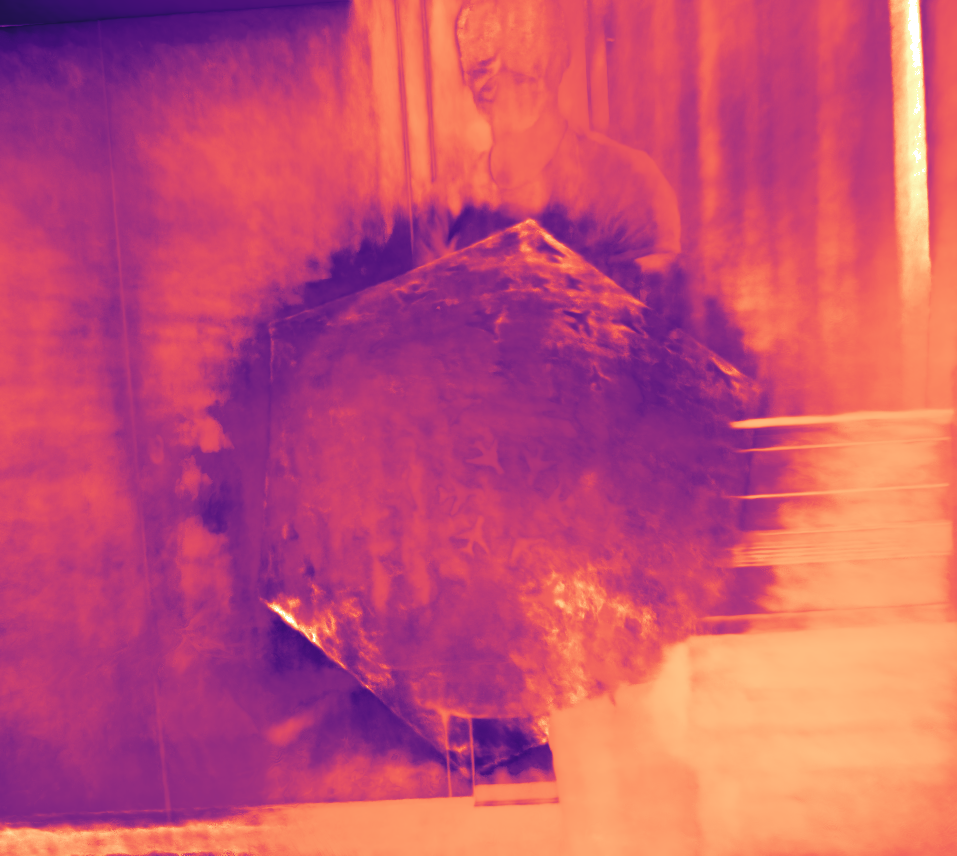
\includegraphics[width=\linewidth,valign=m]{figs/depth_compare_big/umbrella/umbrella_enerfie_depth.png} & 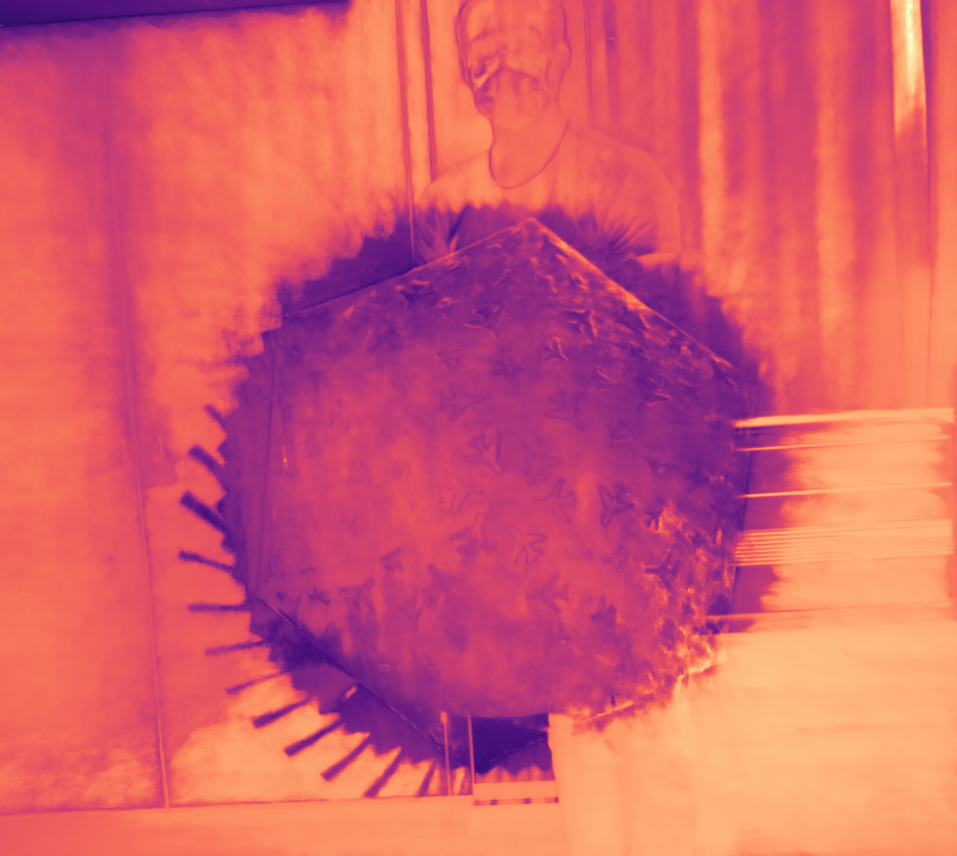
\includegraphics[width=\linewidth,valign=m]{figs/depth_compare_big/umbrella/umbrella_depth_nerfies.png} & 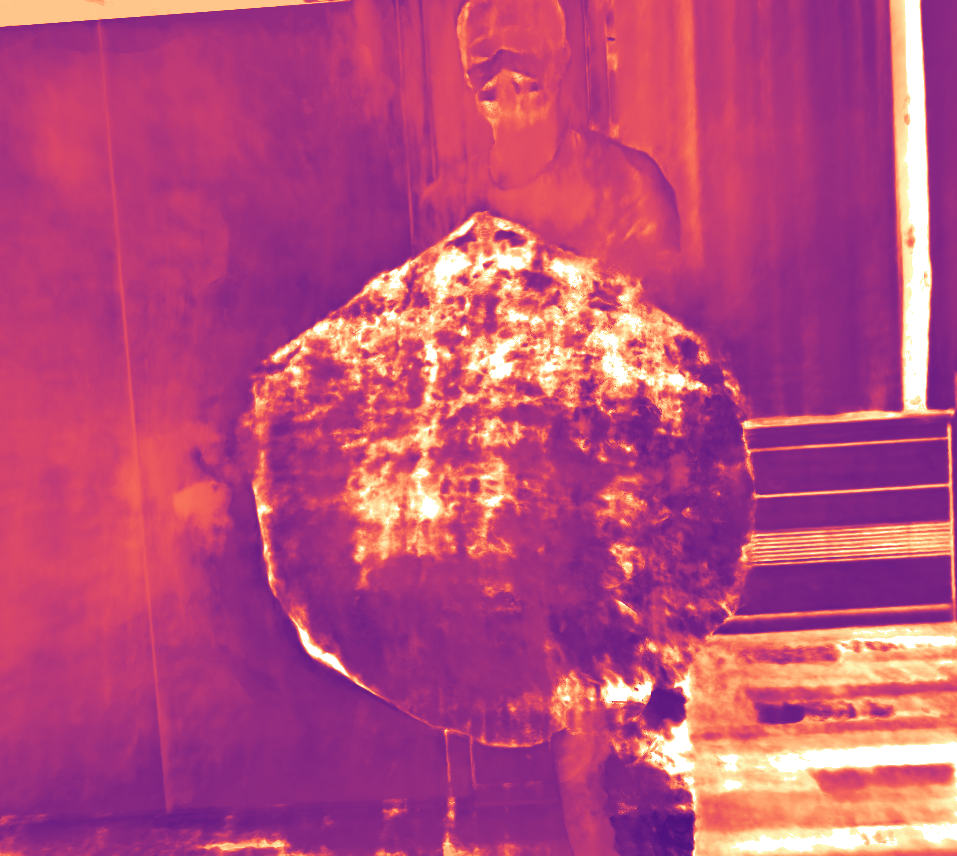
\includegraphics[width=\linewidth,valign=m]{figs/depth_compare_big/umbrella/umbrella_hypernerf.png}   \\

\vspace{0.1cm}
\rotatebox{90}{Candle} & 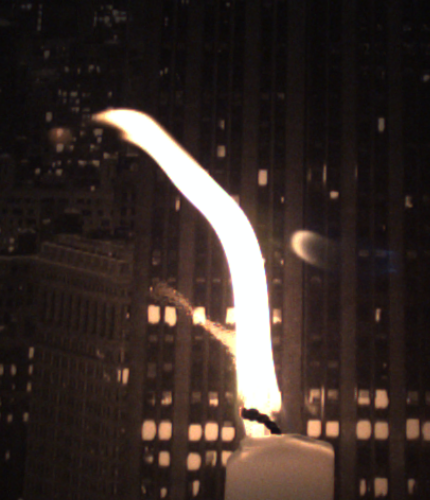
\includegraphics[width=\linewidth,valign=m]{figs/depth_compare_big/candle/000529.png} & 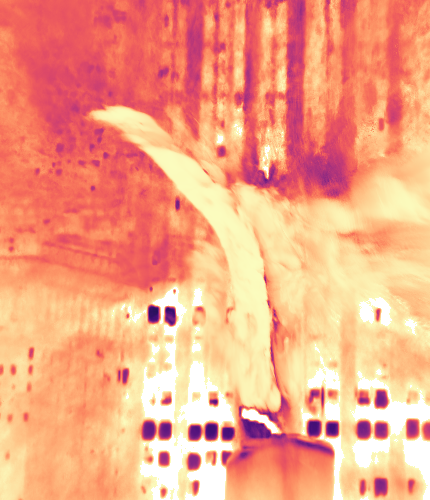
\includegraphics[width=\linewidth,valign=m]{figs/depth_compare_big/candle/candle_depth_ours.png} & 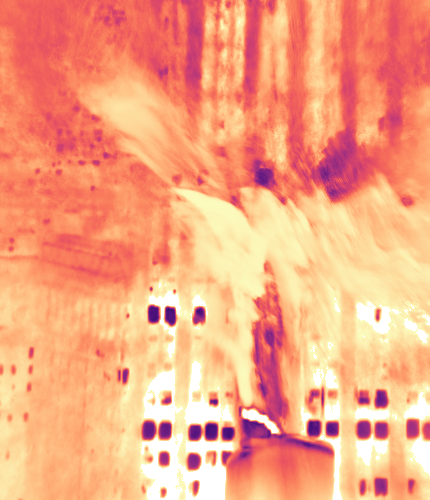
\includegraphics[width=\linewidth,valign=m]{figs/depth_compare_big/candle/candle_depth_enerfie.png} & 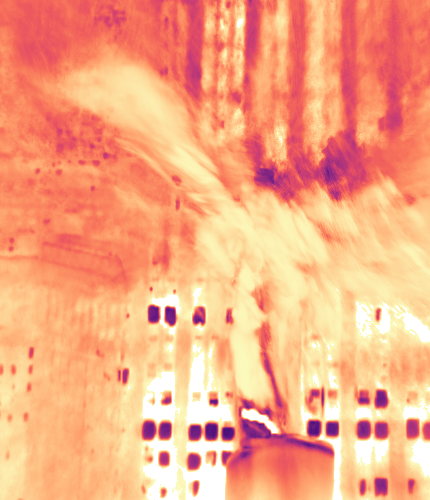
\includegraphics[width=\linewidth,valign=m]{figs/depth_compare_big/candle/candle_depth_nerfie.png} & 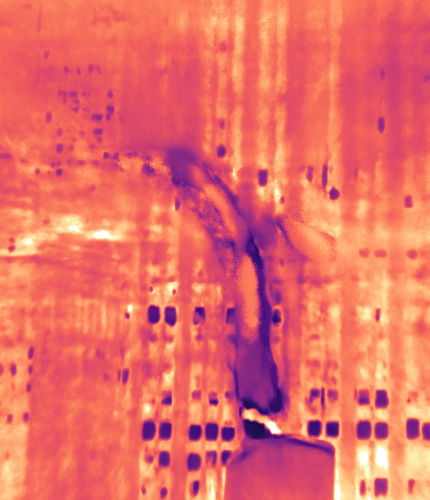
\includegraphics[width=\linewidth,valign=m]{figs/depth_compare_big/candle/candle_depth_hypernerf.png}   \\
\vspace{0.1cm}

\rotatebox{90}{Fountain} & 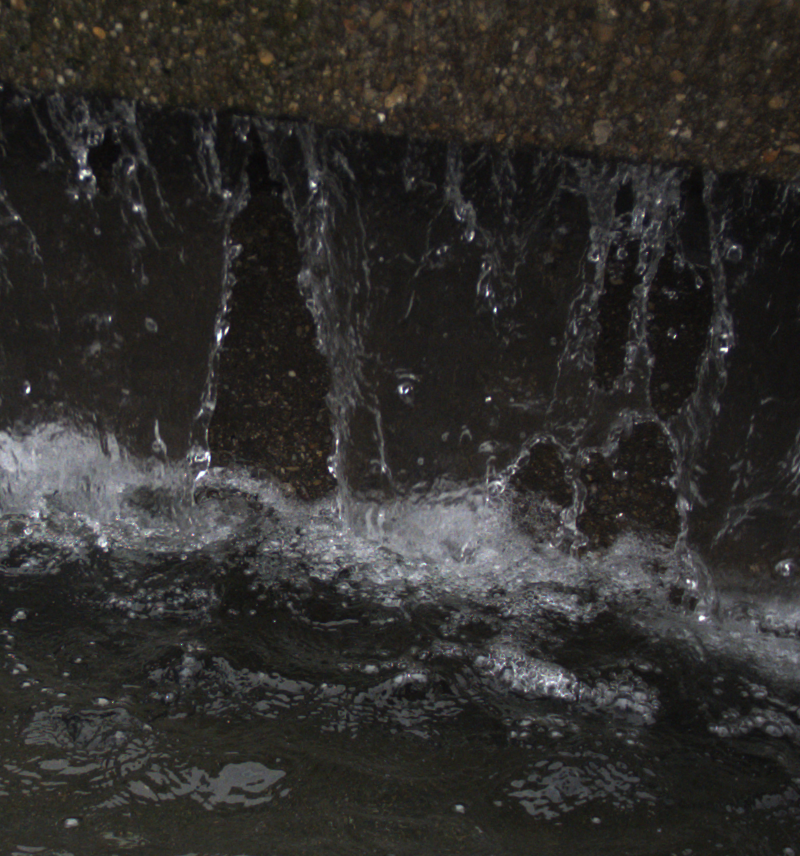
\includegraphics[width=\linewidth,valign=m]{figs/depth_compare_big/fountain/000506.png} & 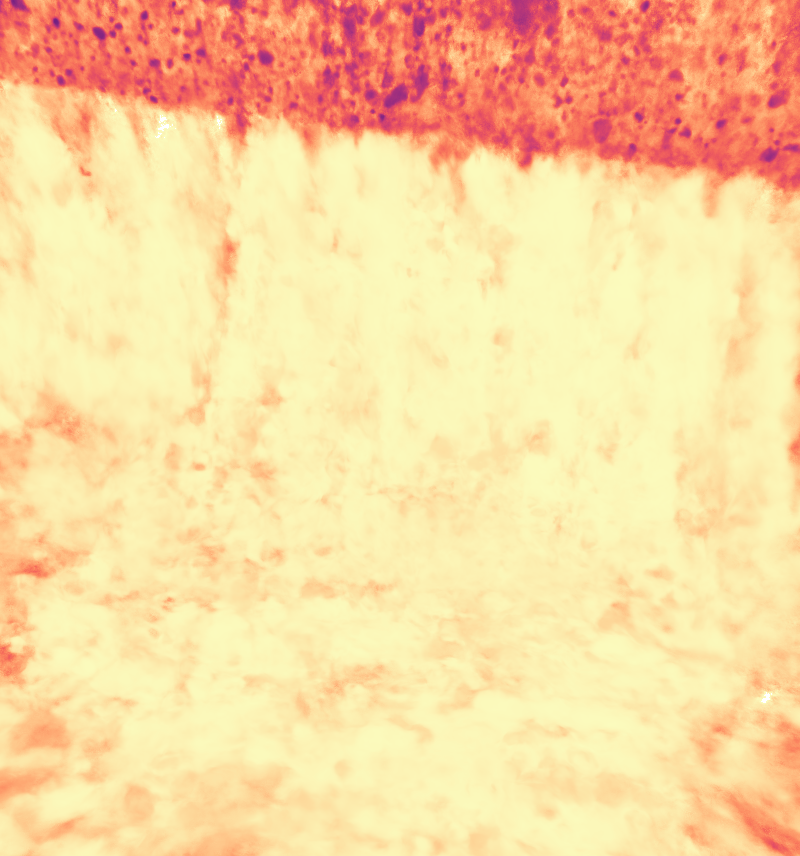
\includegraphics[width=\linewidth,valign=m]{figs/depth_compare_big/fountain/fountain_depth_denerf.png} & 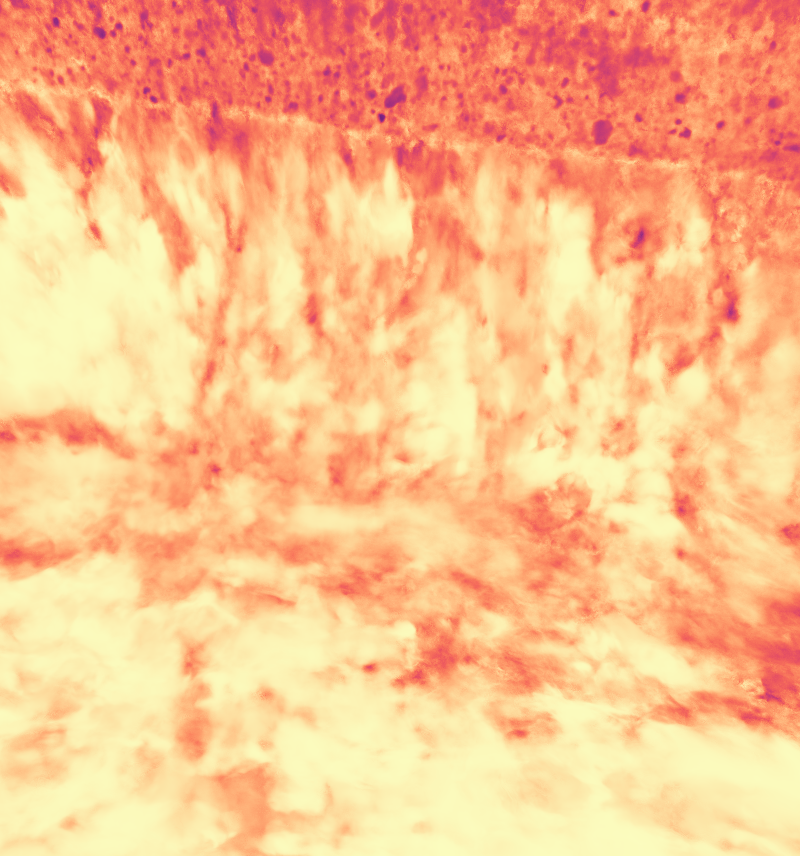
\includegraphics[width=\linewidth,valign=m]{figs/depth_compare_big/fountain/fountain_enerfie_depth.png} & 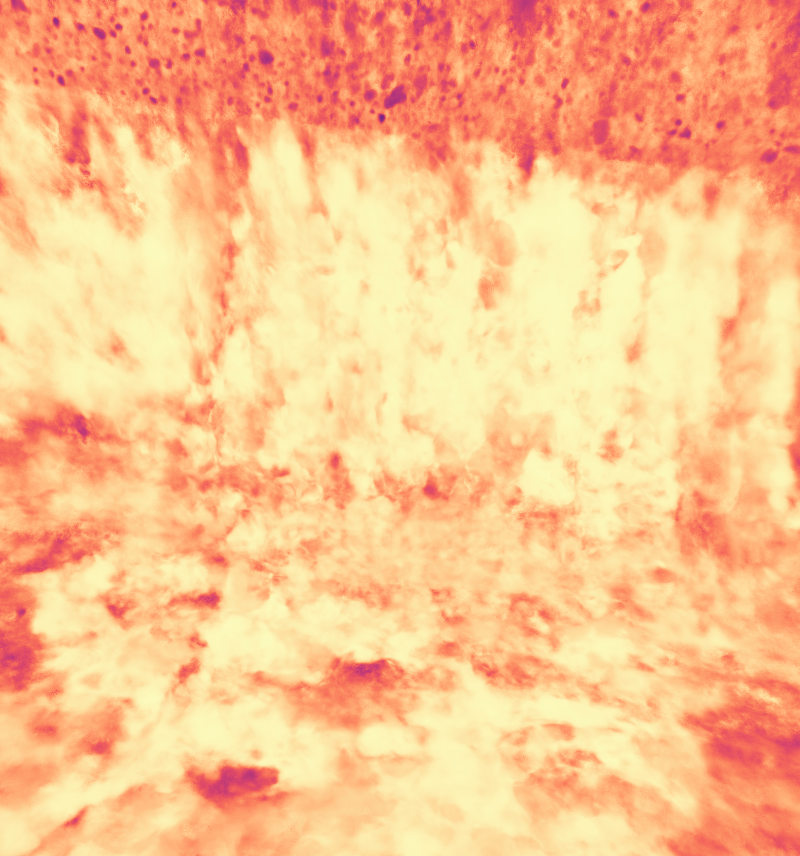
\includegraphics[width=\linewidth,valign=m]{figs/depth_compare_big/fountain/fountain_depth_nerfies.png} & 
\includegraphics[width=\linewidth,valign=m]{figs/depth_compare_big/fountain/fountain_hypernerf.png}  \\

\vspace{0.1cm}
% \noalign{\vspace{3pt}}
\rotatebox{90}{Selfie} & 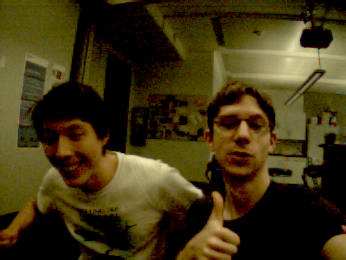
\includegraphics[width=\linewidth,valign=m]{figs/depth_compare_big/selfie/000208.png} & 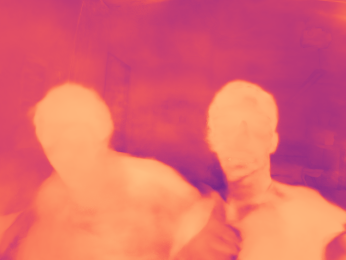
\includegraphics[width=\linewidth,valign=m]{figs/depth_compare_big/selfie/selfie_denerf_depth_208.png} & 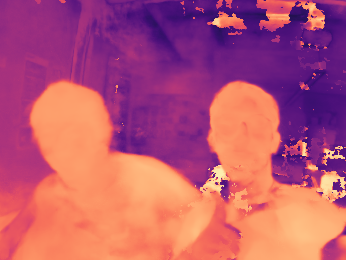
\includegraphics[width=\linewidth,valign=m]{figs/depth_compare_big/selfie/selfie_enerfie_depth_208.png} & 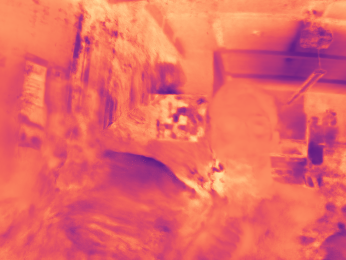
\includegraphics[width=\linewidth,valign=m]{figs/depth_compare_big/selfie/selfie_nerfies_depth.png} & 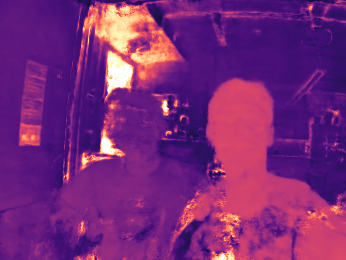
\includegraphics[width=\linewidth,valign=m]{figs/depth_compare_big/selfie/selfie_hypernerf_depth.png} \\

\vspace{0.1cm}
% \noalign{\vspace{3pt}}
\rotatebox{90}{Toycar} &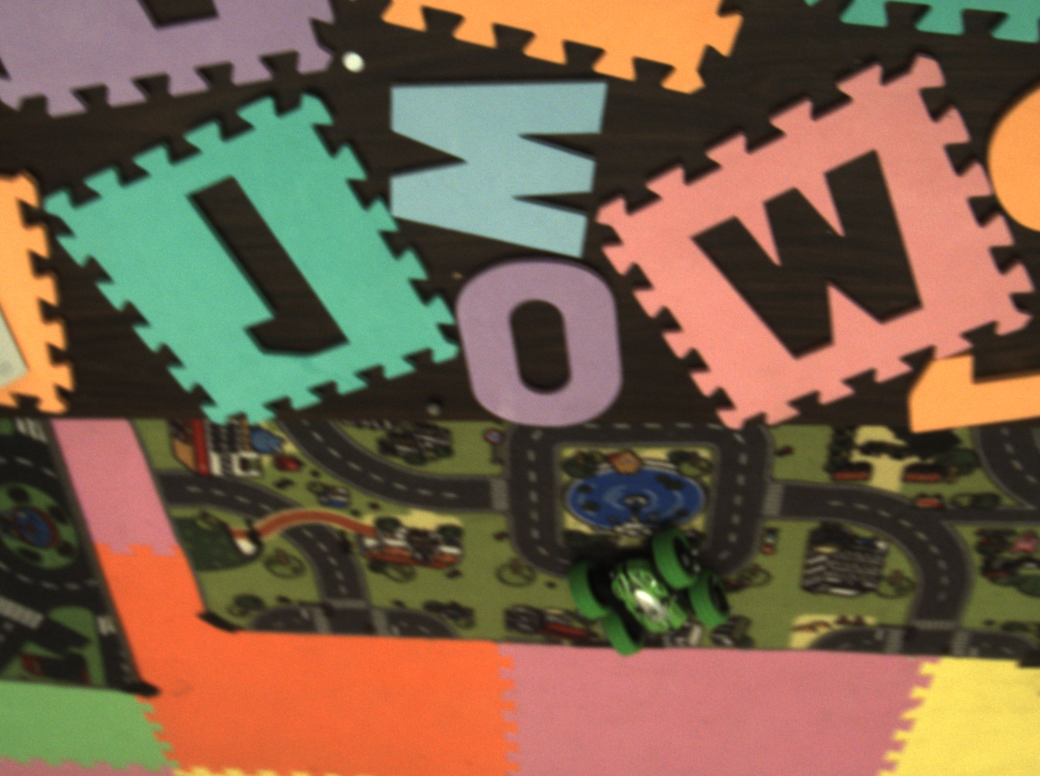
\includegraphics[width=\linewidth,valign=m]{figs/depth_compare_big/toycar/000030.png} & 
\includegraphics[width=\linewidth,valign=m]{figs/depth_compare_big/toycar/toycar_denerf_depth.png} & 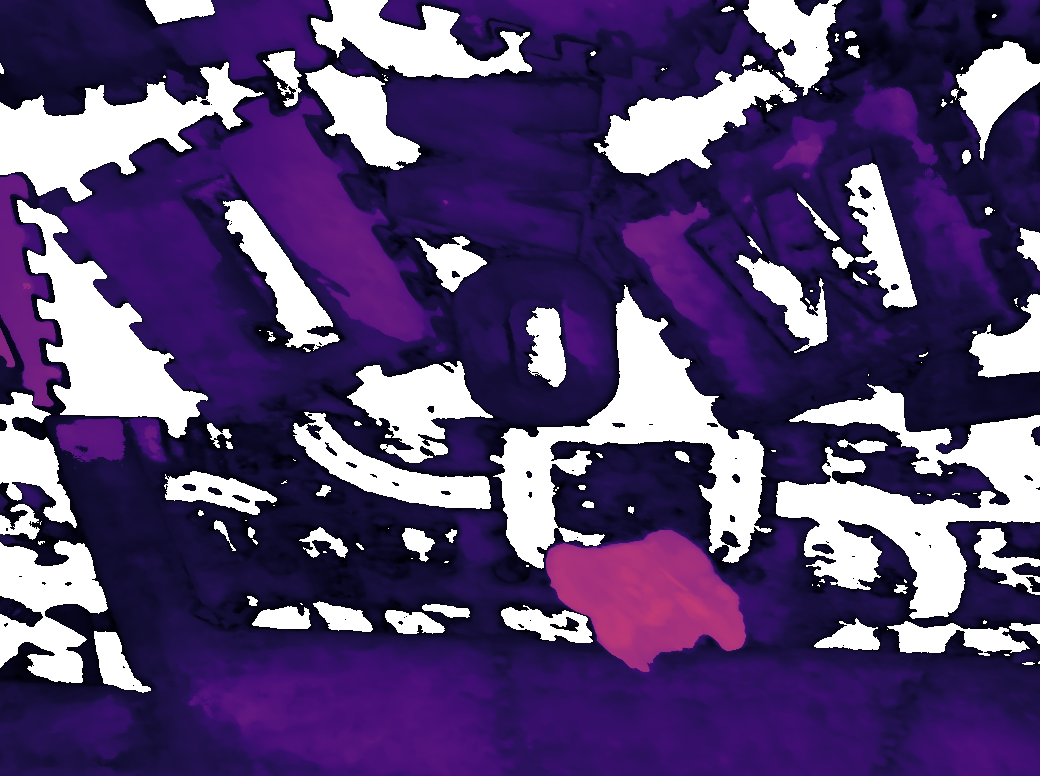
\includegraphics[width=\linewidth,valign=m]{figs/depth_compare_big/toycar/toycar_enerfie_depth.png} & 
\includegraphics[width=\linewidth,valign=m]{figs/depth_compare_big/toycar/toycar_nerfies_depth.png} & 
\includegraphics[width=\linewidth,valign=m]{figs/depth_compare_big/toycar/toycar_hypernerf_depth.png}  \\

% \noalign{\vspace{3pt}}
\rotatebox{90}{UAV} & 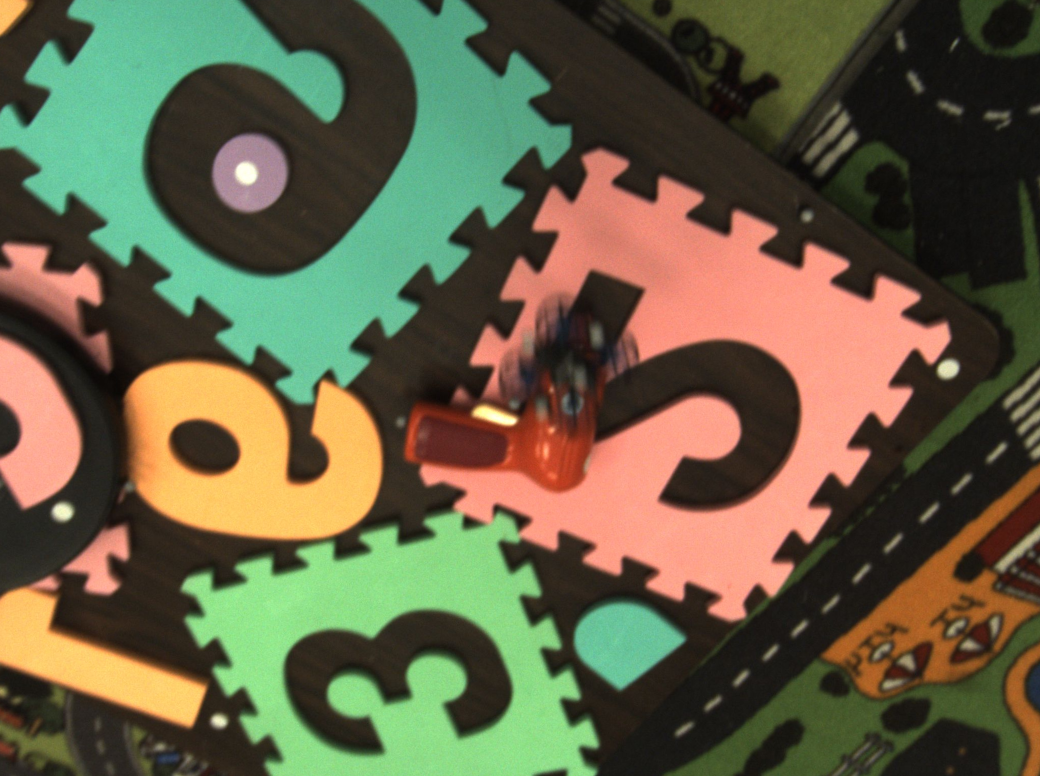
\includegraphics[width=\linewidth,valign=m]{figs/depth_compare_big/uav/000027_gt.png} & 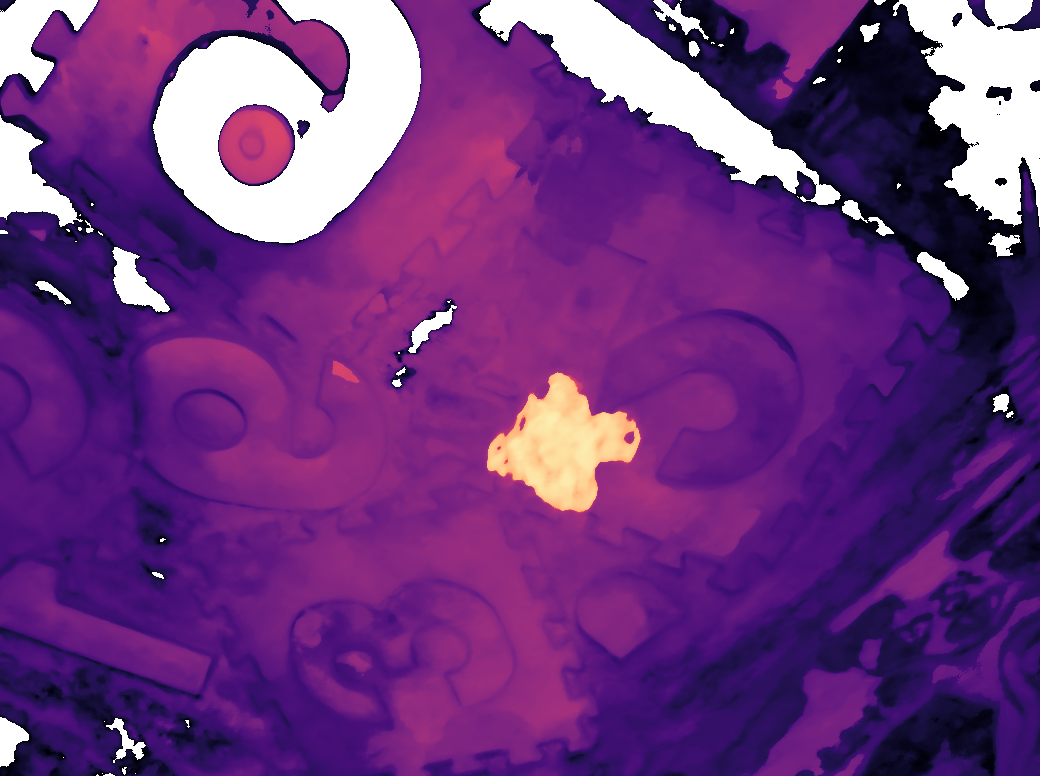
\includegraphics[width=\linewidth,valign=m]{figs/depth_compare_big/uav/uav_denerf_depth.png} & 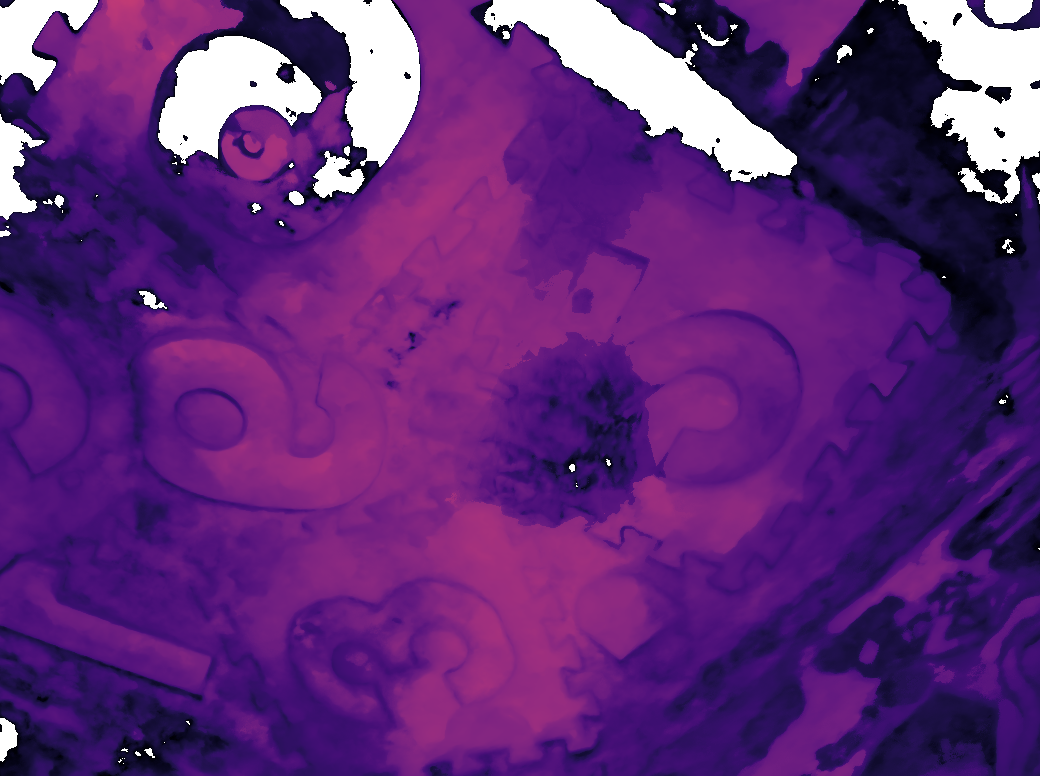
\includegraphics[width=\linewidth,valign=m]{figs/depth_compare_big/uav/uav_enerfie_depth.png} & 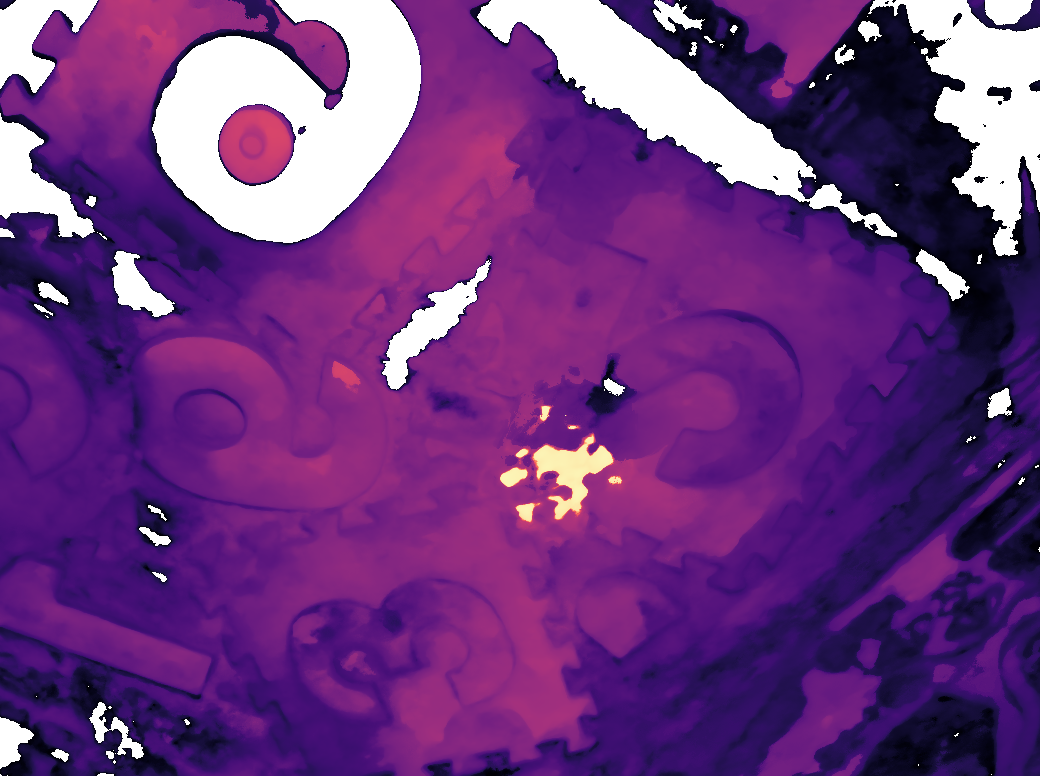
\includegraphics[width=\linewidth,valign=m]{figs/depth_compare_big/uav/uav_nerfies_depth.png} & 
\includegraphics[width=\linewidth,valign=m]{figs/depth_compare_big/uav/uav_hypernerf_depth.png} \\

% \noalign{\vspace{3pt}}
 & RGB & DE-NeRF(Ours) & DE-Baseline & Nerfies~\cite{park2021nerfies} & HyperNeRF~\cite{park2021hypernerf} 
\end{tabular}
\end{center}
\vspace{-0.2cm}
\caption{Qualitative depth comparisons of our method against other methods on synthetic and real-world datasets.}
\label{fig:qualitative results rgb}
\end{table*}




\subsection{ Sensitivity to Hyperparameter $\lambda$}
In Table ~\ref{tab:lambda_compare} we analyze how the hyperparameters $\lambda_rgb$ impact the performance. It can be noticed that with small $\lambda_rgb$ the method may suffer due to color confusion caused by noisy brightness estimation. Similarly, the PSNR drops when $\lambda_rgb$ is too large as the event information cannot be fully exploited. Nevertheless, our experiments show that the proposed method is not too sensitive to the choice of the hyperparameter $\lambda$.





\section{Translation vs. SE(3)  Deformation Field}
As suggested in~\cite{park2021nerfies}, we also experimented with SE(3)  deformation field, separately from the translation-only deformation field reported in the paper.
We found that SE(3) field occasionally performs better than that of translation only. These examples are Fluid and Umbrella. Therefore, the qualitative results in the supplementary material for the latter example are shown with SE(3) deformation field. These two cases can be directly compared in Table 4 (in the paper) and Table~\ref{fig:qualitative results rgb} (here) for the mentioned examples. Some quantitative results for translation only and SE(3) deformation field are reported in Table~\ref{tab:rotation_compare}. It can be seen that the SE(3) deformation is not always better. Therefore, we reported translation-only deformation field results in the main paper, for simplicity. 


%In this section, we discuss the influence of using different deformation approaches in the Lego and Umbrella sequence. The Lego movement is induced with two links on revolute joints and the rotating umbrella shows a typical rotation movement about the center shaft. We observe that as \cite{park2021nerfies} argued the SE3 deformation approach yields better results because learning the same rotation parameters across the space makes optimization easier. However, for more complex motions like in Lego, the translation deformation performs slightly better because it has less freedom movement to optimize.




\section{More Qualitative Results}

We present more qualitative results for our method and comparison with other methods Figure \ref{fig:qualitative results rgb}.  Please, also refer to our supplementary video. 



\begin{comment}
\todo[inline]{Possible questions}
\begin{itemize}
    \item \textcolor{blue}{Limitations }
    \item \textcolor{blue}{Training details }
    \item \textcolor{blue}{Hyperparameters }
    \item \textcolor{blue}{How to deal with real noisy data }
    \item \textcolor{blue}{Details of PoseNet}
    \item \textcolor{blue}{Details of Loss function}
    \item \textcolor{blue}{Inference time}
    \item \textcolor{blue}{Different warp compare}
    \item \textcolor{blue}{Why not use interpolate intensity to train}
    \item \textcolor{blue}{The detail of simulate fire and water dataset}
    \item \textcolor{blue}{Depth accuracy}    
\end{itemize}

\end{comment}













    
   













{\small
\bibliographystyle{ieee_fullname}
\bibliography{11_references}
}

\end{document}
